\documentclass[12pt]{article}
\usepackage{ucs}
\usepackage[T1,T2A]{fontenc}
\usepackage[utf8]{inputenc}  % Включаем поддержку UTF8
\usepackage[russian]{babel}  % Включаем пакет для поддержки русского языка
\title{is8-facts-lang-model}
\date{mar 2019}
\author{Anthony Belyaev}
 
\usepackage{geometry} % А4, примерно 28-31 строк(а) на странице	
    \geometry{paper=a4paper}
    \geometry{includehead=false} % Нет верх. колонтитула
    \geometry{includefoot=true}  % Есть номер страницы
    \geometry{bindingoffset=0mm} % Переплет    : 0  мм
    \geometry{top=20mm}          % Поле верхнее: 20 мм
    \geometry{bottom=25mm}       % Поле нижнее : 25 мм 
    \geometry{left=25mm}         % Поле левое  : 25 мм
    \geometry{right=25mm}        % Поле правое : 25 мм
    \geometry{headsep=10mm}  % От края до верх. колонтитула: 10 мм
    \geometry{footskip=20mm} % От края до нижн. колонтитула: 20 мм 
\usepackage{amsmath}    % \bar    (матрицы и проч. ...)
\usepackage{amsfonts}   % \mathbb (символ для множества действительных чисел и проч. ...)
\usepackage{mathtools}  % \abs, \norm
    \DeclarePairedDelimiter\abs{\lvert}{\rvert}
    \DeclarePairedDelimiter\norm{\lVert}{\rVert}
\usepackage{listings} %листинги

\usepackage{minted}

\newenvironment{comment}{}{}	%многострочные комментарии

\usepackage{graphicx}	%картинки
\graphicspath{ {img/} }	%папка с картинками

\usepackage{listings}
 \usepackage{color}
\definecolor{pblue}{rgb}{0.13,0.13,1}
\definecolor{pgreen}{rgb}{0,0.5,0}
\definecolor{pred}{rgb}{0.9,0,0}
\definecolor{pgrey}{rgb}{0.46,0.45,0.48}
\definecolor{deepblue}{rgb}{0,0,0.5}
\definecolor{deepred}{rgb}{0.6,0,0}
\definecolor{deepgreen}{rgb}{0,0.5,0}

\lstset{
    tabsize=4,
  language=C++,
  captionpos=b,
  tabsize=3,
  frame=lines,
  numbers=left,
  numberstyle=\tiny,
  numbersep=5pt,
  breaklines=true,
  showstringspaces=false,
  basicstyle=\footnotesize,
%  identifierstyle=\color{magenta},
  keywordstyle=\color[rgb]{0,0,1},
  commentstyle=\color{green},
  stringstyle=\color{red}
  }

\begin{comment}
 %для подсветки листинга javascript
 \usepackage{color}
\definecolor{lightgray}{rgb}{.9,.9,.9}
\definecolor{darkgray}{rgb}{.4,.4,.4}
\definecolor{purple}{rgb}{0.65, 0.12, 0.82}

\lstdefinelanguage{JavaScript}{
  keywords={typeof, new, true, false, catch, function, return, null, catch, switch, var, if, in, while, do, else, case, break},
  keywordstyle=\color{blue}\bfseries,
  ndkeywords={class, export, boolean, throw, implements, import, this},
  ndkeywordstyle=\color{darkgray}\bfseries,
  identifierstyle=\color{black},
  sensitive=false,
  comment=[l]{//},
  morecomment=[s]{/*}{*/},
  commentstyle=\color{purple}\ttfamily,
  stringstyle=\color{red}\ttfamily,
  morestring=[b]',
  morestring=[b]"
}

\lstset{
   language=JavaScript,
   %backgroundcolor=\color{lightgray},
   extendedchars=true,
   basicstyle=\footnotesize\ttfamily,
   showstringspaces=false,
   showspaces=false,
   %numbers=left,
   %numberstyle=\footnotesize,
   %numbersep=9pt,
   %tabsize=2,
   breaklines=true,
   showtabs=false,
   captionpos=b
}
\end{comment}


\begin{document}
    \newpage
    {
        \thispagestyle{empty}
        \centering
        
        \textbf{
        МОСКОВСКИЙ ГОСУДАРСТВЕННЫЙ ТЕХНИЧЕСКИЙ УНИВЕРСИТЕТ ИМЕНИ Н. Э. БАУМАНА \\
        Факультет информатики и систем управления \\
        Кафедра теоретической информатики и компьютерных технологий}
        \bigskip
        \bigskip
        \bigskip
        \bigskip
        \bigskip
        \bigskip
        \vfill

        {\large Лабораторная работа №910}\\
        по курсу <<Информационный поиск>>\\
	\LARGE{<<Page Rank>> }
	\normalsize

        \bigskip
        \vfill
        \hfill\parbox{5cm} {
            Выполнил:\\
            студент группы ИУ9-21М \hfill \\
            Беляев А. В.\hfill \medskip\\
            Проверила:\\
            Лукашевич Н. В.\hfill
        }
        \vspace{\fill}

        
        Москва \number\year
        \clearpage
    }
	\newpage
	
    {
        \section{Цель работы}
    }
	
    Вычислить PageRank для сетей на Рис. \ref{lab9} и \ref{lab10}.

    В ходе работы необходимо перемножать вектор исходных состояний (которые равновероятны) и матрицу переходов до схождения, либо итеративно N раз. В ходе работы был реализован алгоритм на N итераций.
    
    Коэффициент телепортации = 0.1
   
   
   {
        \section{Текст программы}
    }
    
% \begin{lstlisting}[language=Python, caption=Исходный код программы]
\begin{minted}[%
 breaklines,
 mathescape,
 linenos,
 numbersep=5pt,
 frame=single]{python}
import numpy as np

np.set_printoptions(precision=3)

ITERATIONS = 5  # it doesnt matter how many iterations
TELEPORT = 0.1


def make_transition_matrix(N, matrix):
    i = 0
    while i < len(matrix):
        row = matrix[i]

        num_of_links = row.count(1)
        if 0 != num_of_links:
            # Нормализовать в строке единицы, поделив на кол-во единиц
            row = [x / num_of_links for x in row]
            # Единицы умножить на коэффициент сглаживания (1-d)
            row = [x * (1 - TELEPORT) for x in row]
            # Ко всем элементам добавить коэффициент (d/N)
            row = [x + (TELEPORT / N) for x in row]
        else:
            # Если со страницы не было ссылок, столбцам ставим 1/N
            row = [1 / N for x in row]

        matrix[i] = row
        i += 1
    return matrix


def pagerank(N: int, matrix: list):
    vector = [1] * N
    v = np.array([x / len(vector) for x in vector])

    matrix = np.array(matrix)
    i = 0
    while i < ITERATIONS:
        v = np.matmul(v, matrix)
        i += 1
    return v


def lab9():
    N_states = 3
    init_matrix = [[0, 1, 1],
                   [0, 0, 1],
                   [0, 1, 0]]
    print('\ninit matrix:')
    print(np.array(init_matrix))

    transition_matrix = make_transition_matrix(N_states, init_matrix)
    print('\ntransition matrix:')
    print(np.array(transition_matrix))

    pr = pagerank(N_states, transition_matrix)
    print('\npagerank:')
    print(np.array(pr))


def lab10():
    N_states = 8
    init_matrix = [[0, 1, 1, 1, 0, 0, 0, 0],  # home
                   [1, 0, 0, 0, 0, 0, 0, 0],  # about
                   [1, 0, 0, 0, 0, 0, 0, 0],  # prod
                   [1, 0, 0, 0, 1, 1, 1, 1],  # links
                   [0, 0, 0, 0, 0, 0, 0, 0],  # ext A
                   [0, 0, 0, 0, 0, 0, 0, 0],  # ext B
                   [0, 0, 0, 0, 0, 0, 0, 0],  # ext C
                   [0, 0, 0, 0, 0, 0, 0, 0]]  # ext D
    print('\ninit matrix:')
    print(np.array(init_matrix))

    transition_matrix = make_transition_matrix(N_states, init_matrix)
    print('\ntransition matrix:')
    print(np.array(transition_matrix))

    pr = pagerank(N_states, transition_matrix)
    print('\npagerank:')
    print(np.array(pr))


if __name__ == '__main__':
    lab9()
    lab10()
\end{minted}
  
    
    {
       \section{Результаты работы}
        
    }
    
    В ходе работы программы были получены следующие матрицы переходов и значения PageRank в Л.Р.9:
    
    
           \begin{figure}
\centering
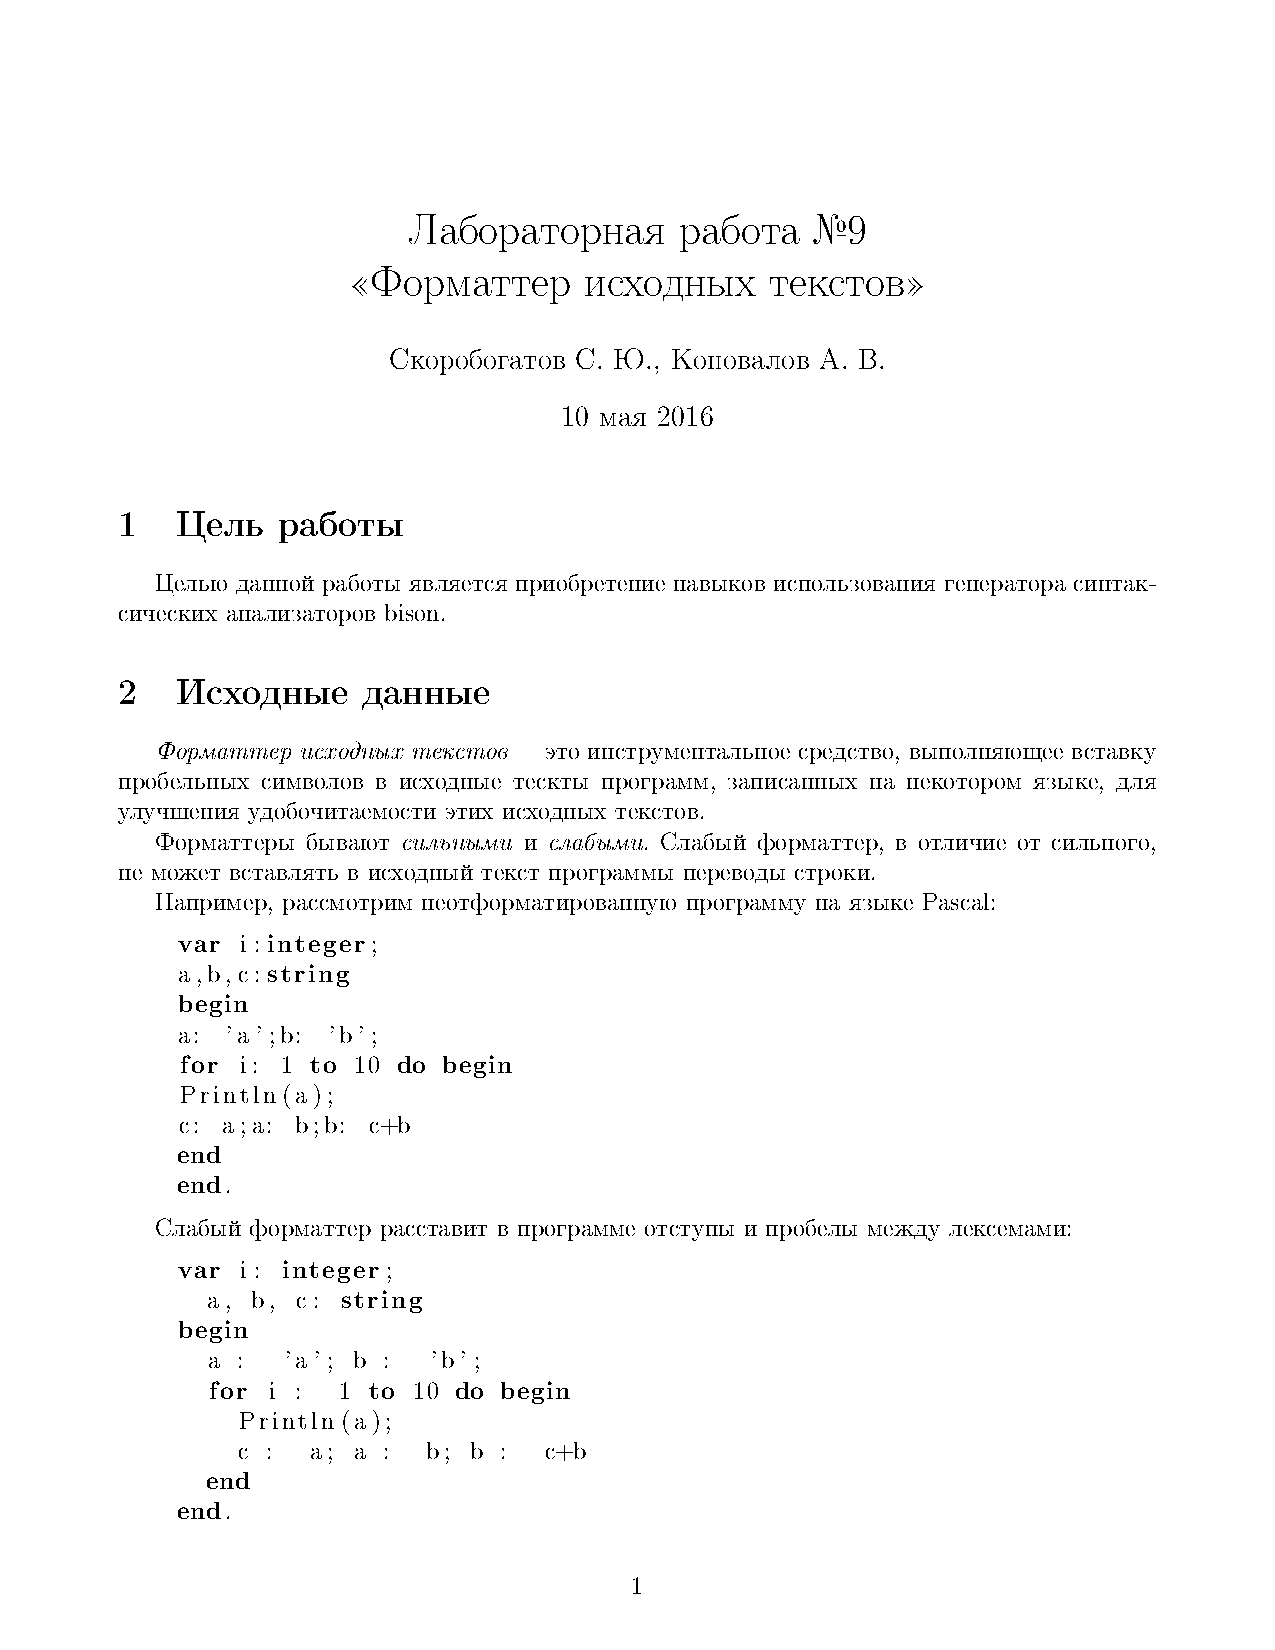
\includegraphics[width=0.3\textwidth]{lab9.png}
\caption{Л.Р.9}
\label{lab9}
\end{figure}
    
    \begin{minted}[%
 breaklines,
 mathescape,
 linenos,
 numbersep=5pt,
 frame=single]{python}
init matrix:
[[0 1 1]
 [0 0 1]
 [0 1 0]]

transition matrix:
[[0.033 0.483 0.483]
 [0.033 0.033 0.933]
 [0.033 0.933 0.033]]

pagerank:
[0.033 0.483 0.483]
 \end{minted}
 

 
 Для Л.Р.10 результаты следующие:
    
    \begin{minted}[%
 breaklines,
 mathescape,
 linenos,
 numbersep=5pt,
 frame=single]{python}
init matrix:
[[0 1 1 1 0 0 0 0]
 [1 0 0 0 0 0 0 0]
 [1 0 0 0 0 0 0 0]
 [1 0 0 0 1 1 1 1]
 [0 0 0 0 0 0 0 0]
 [0 0 0 0 0 0 0 0]
 [0 0 0 0 0 0 0 0]
 [0 0 0 0 0 0 0 0]]

transition matrix:
[[0.013 0.312 0.312 0.312 0.013 0.013 0.013 0.013]
 [0.912 0.013 0.013 0.013 0.013 0.013 0.013 0.013]
 [0.912 0.013 0.013 0.013 0.013 0.013 0.013 0.013]
 [0.193 0.013 0.013 0.013 0.193 0.193 0.193 0.193]
 [0.125 0.125 0.125 0.125 0.125 0.125 0.125 0.125]
 [0.125 0.125 0.125 0.125 0.125 0.125 0.125 0.125]
 [0.125 0.125 0.125 0.125 0.125 0.125 0.125 0.125]
 [0.125 0.125 0.125 0.125 0.125 0.125 0.125 0.125]]

pagerank:
[0.333 0.13  0.13  0.13  0.069 0.069 0.069 0.069]
 \end{minted}
    	
    	
   \begin{figure}
\centering
\includegraphics[width=0.6\textwidth]{lab10.png}
\caption{Л.Р.10}
\label{lab10}
\end{figure}
    	
    	
        {
       \section {Выводы}
        
    }
        
        В ходе работы была изучена и реализована популярная моедль ранжирования -- PageRank.
   
    \end{document}
    
